\section{Combinazione agli SLE quasi permanente}
La $[2.5.4]$ del \emph{decreto 17 gennaio 2018} definisce la combinazione quasi permanente come quella impiegata per gli effetti a lungo termine, in cui
\[
	G_1 + G_2 + \psi_{21}\cdot Q_{1k} + \psi_{22}\cdot Q_{2k} + \psi_{23}\cdot Q_{3k} + \dots
\]

Come si può capire, per gli stati limite di esercizio quasi permanente è presente una sola combinazione di carico

\subsection{Calcolo dell'azione}
L'azione che ne deriva è unica e vale

\begin{align*}
	\begin{cases}
		 Q_{1} &= 8.00+11.52+3.75 + 11.55+7.98+9.20 + 0 + 0.3\cdot(7.50+14.40) + 0 =\\&= 58.57\,\dfrac{kN}{m}\\\\
		 Q_2 &= 8.00+6.72+3.75 + 11.55+4.65+9.20 + 0+ 0.3\cdot(7.50+8.40) + 0 =\\&= 48.64\,\dfrac{kN}{m}\\\\
		 Q_3 &=  8.00+3.20+3.75 + 11.55+2.215+9.20 + 0+ 0.3\cdot(7.50+4.00) + 0 =\\&= 41.365\,\dfrac{kN}{m}
	\end{cases}
\end{align*}
rispettivamente per il primo tratto ($P13\div P16$), per il secondo tratto ($P16\div P17$) e per il terzo tratto di trave ($P17$ - vano scala).

Il diagramma dell'inviluppo è generato da un'unica funzione, essendo $Q_{i,max} = Q_{i,min} = Q_i$ per $i=1,2,3$ tratti della trave, ed è quello descritto in figura~\ref{fig:envelope_sleQP}.

I valori di riferimento sono, come al solito, riportati nelle tabelle~\ref{tab:max_min_bendingMomentEnvelope_sleQP} e \ref{tab:shearEnvelope_sleQP}.

\begin{table}
  	\centering
  	\caption{Valori massimi e minimi dell'inviluppo dei momenti}
  	\label{tab:max_min_bendingMomentEnvelope_sleQP}
  	\begin{tabular}{lcccr}
		\toprule
		& $M_{Ed}^+\,[kN\,m]$ & $s_{max}\,[m]$ & $M_{Ed}^-\,[kN\,m]$ & $s_{min}\,[m]$ \\
		Sezione &             &          &             &          \\
\midrule
C1      &     29.2567 &        1 &         NaN &      NaN \\
N2      &         NaN &      NaN &    -86.4996 &        3 \\
C2      &     58.6555 &     5.23 &           0 &      NaN \\
N3      &         NaN &      NaN &    -90.7684 &      7.5 \\
C3      &     31.0543 &     9.55 &           0 &      NaN \\
N4      &         NaN &      NaN &    -80.7336 &     11.5 \\
C4      &     48.9643 &    13.82 &           0 &      NaN \\
N5      &         NaN &      NaN &    -125.128 &     16.5 \\
C5      &     75.8908 &     19.6 &           0 &      NaN \\
N6      &         NaN &      NaN &    -112.499 &    22.65 \\
C6      &     35.9769 &    25.34 &         NaN &      NaN \\
\bottomrule
	\end{tabular}
  \end{table}
  
\begin{table}
  	\centering
  	\caption{Valori massimi e minimi dell'inviluppo dei tagli}
  	\label{tab:shearEnvelope_sleQP}
  	\begin{tabular}{lcccr}
		\toprule
		& $T_{Ed}^+\,[kN]$ & $s_{max}\,[m]$ & $T_{Ed}^-\,[kN]$ & $s_{min}\,[m]$ \\
		Sezione &             &          &             &          \\
		\midrule
N1      &    84.006 &        0 &         0 &        0 \\
N2      &   185.787 &        3 &  -165.029 &        3 \\
N3      &   170.316 &      7.5 &  -188.546 &      7.5 \\
N4      &   154.466 &     11.5 &  -164.588 &     11.5 \\
N5      &   158.492 &     16.5 &  -173.737 &     16.5 \\
N6      &    133.49 &    22.65 &   -151.89 &    22.65 \\
N7      &         0 &    26.65 &  -66.4499 &    26.65 \\
		\bottomrule
	\end{tabular}
  \end{table}

\begin{figure}
	\centering
	\subfloat[\emph{Diagramma dell'inviluppo dei momenti flettenti}]{
	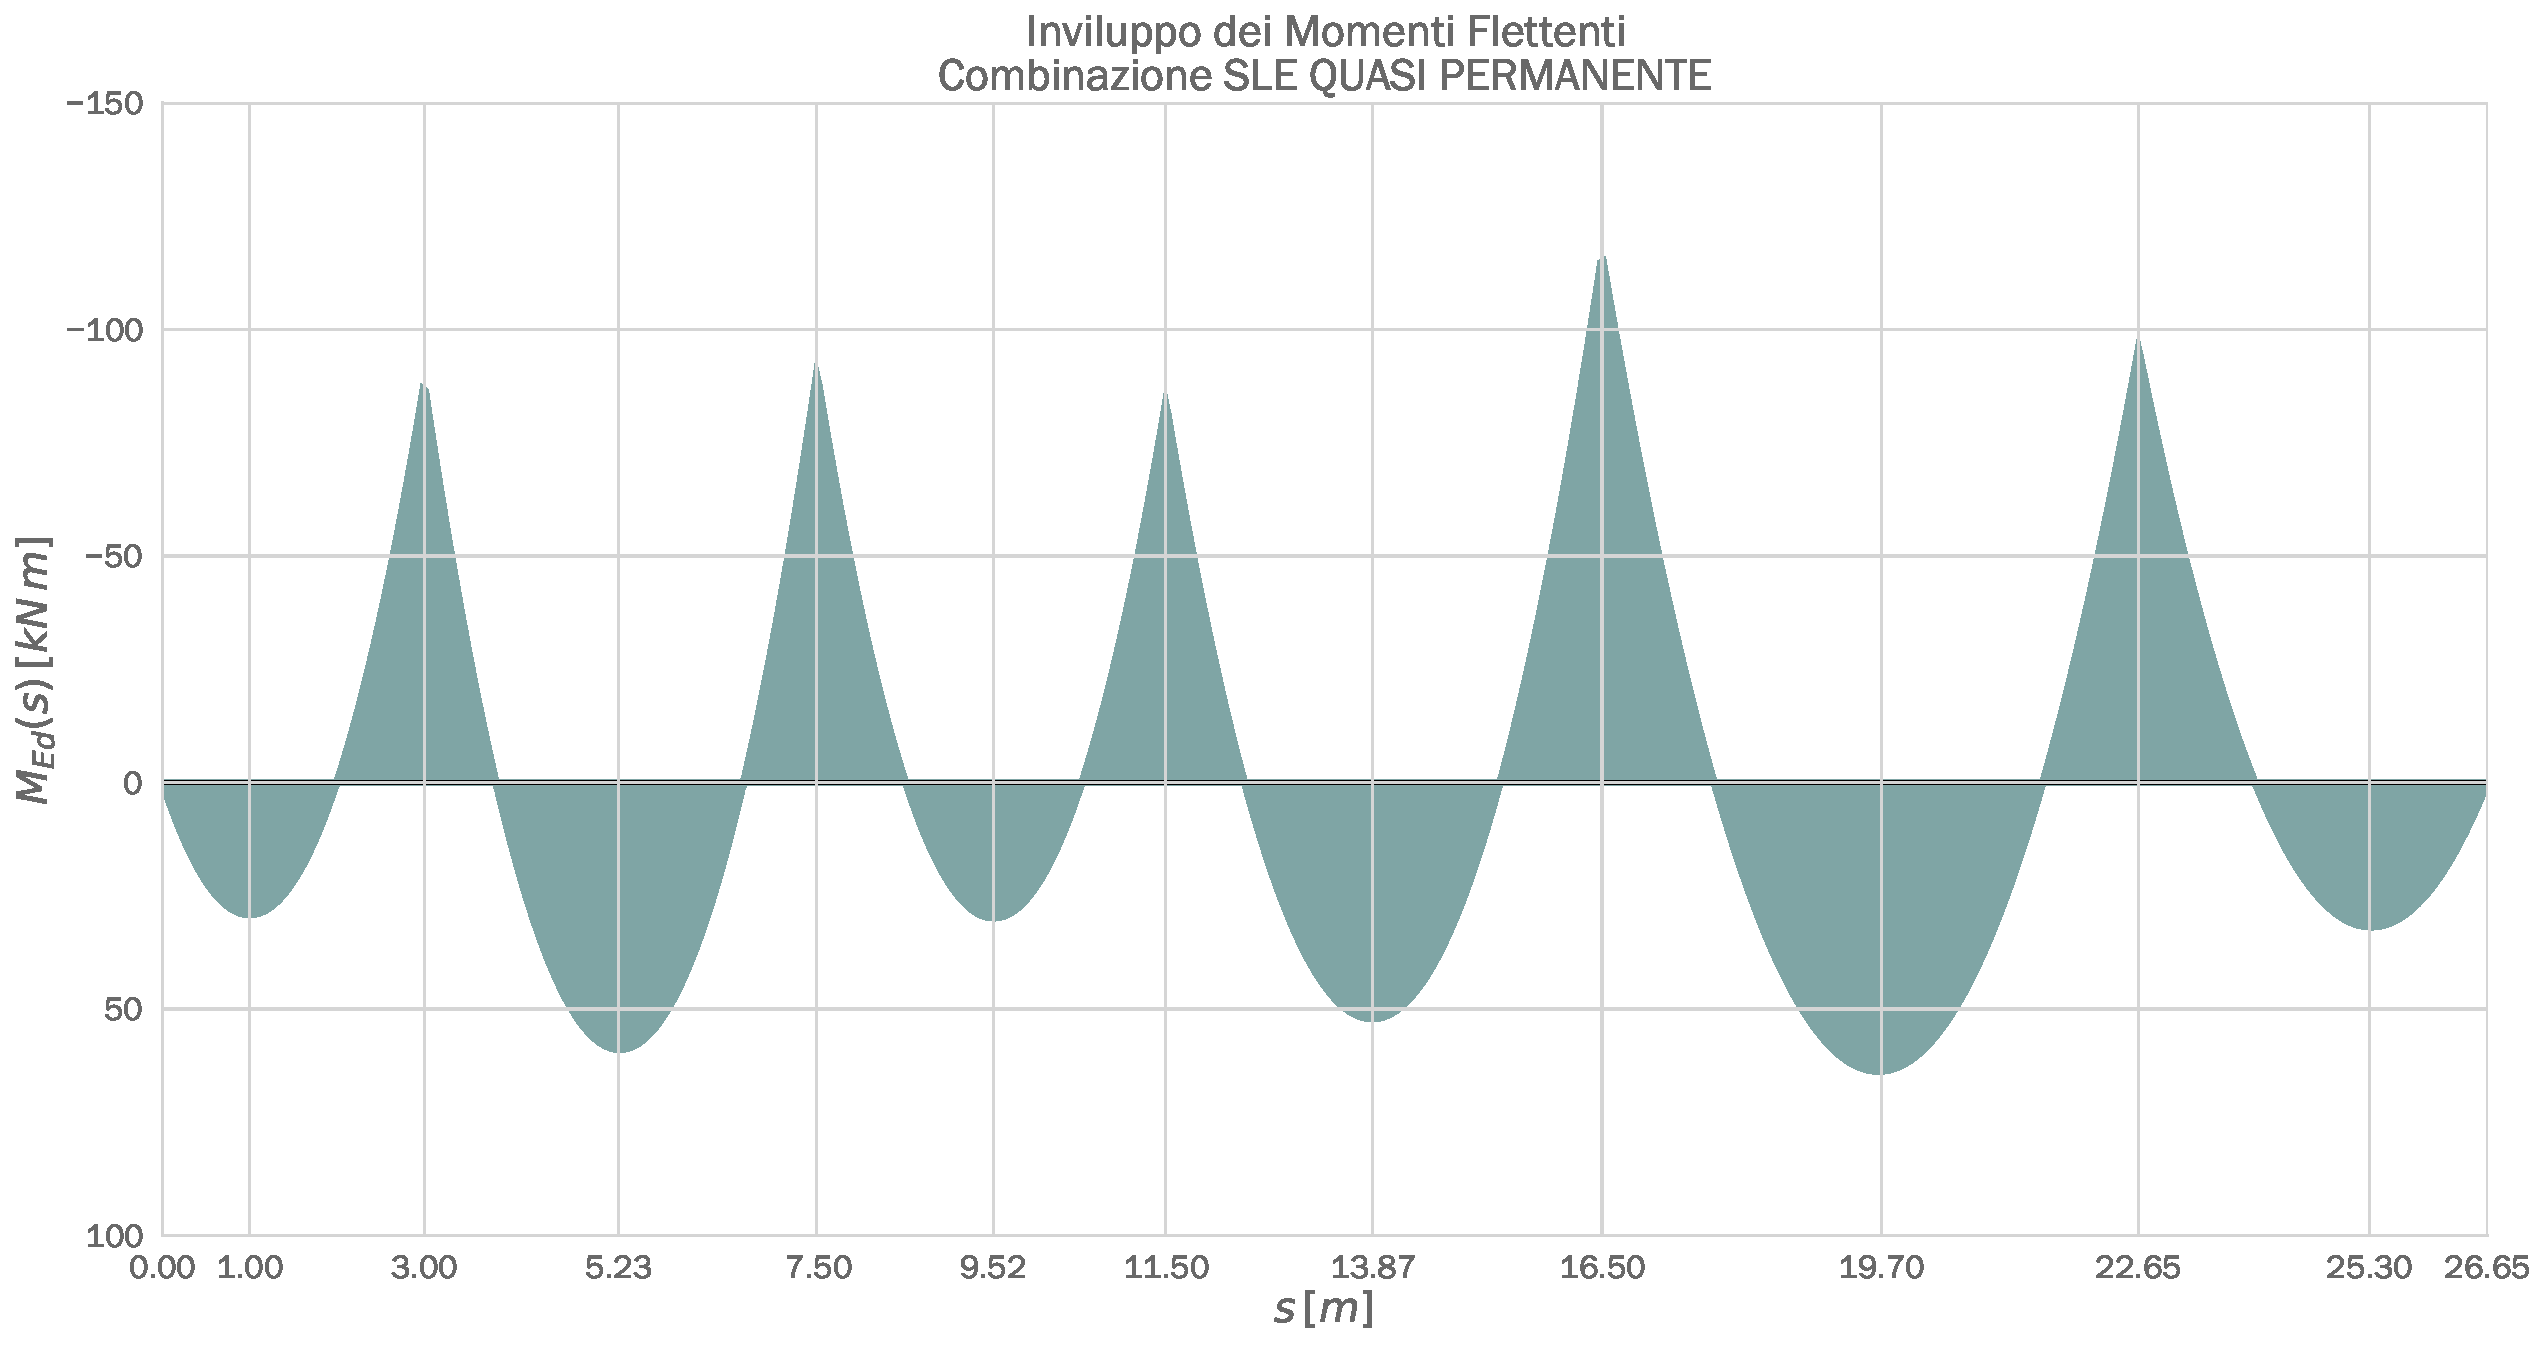
\includegraphics[width=.9\textwidth]{../../export/img/bendingMomentEnvelope_sleQP}}\\
	\subfloat[\emph{Diagramma dell'inviluppo dei tagli}]{
	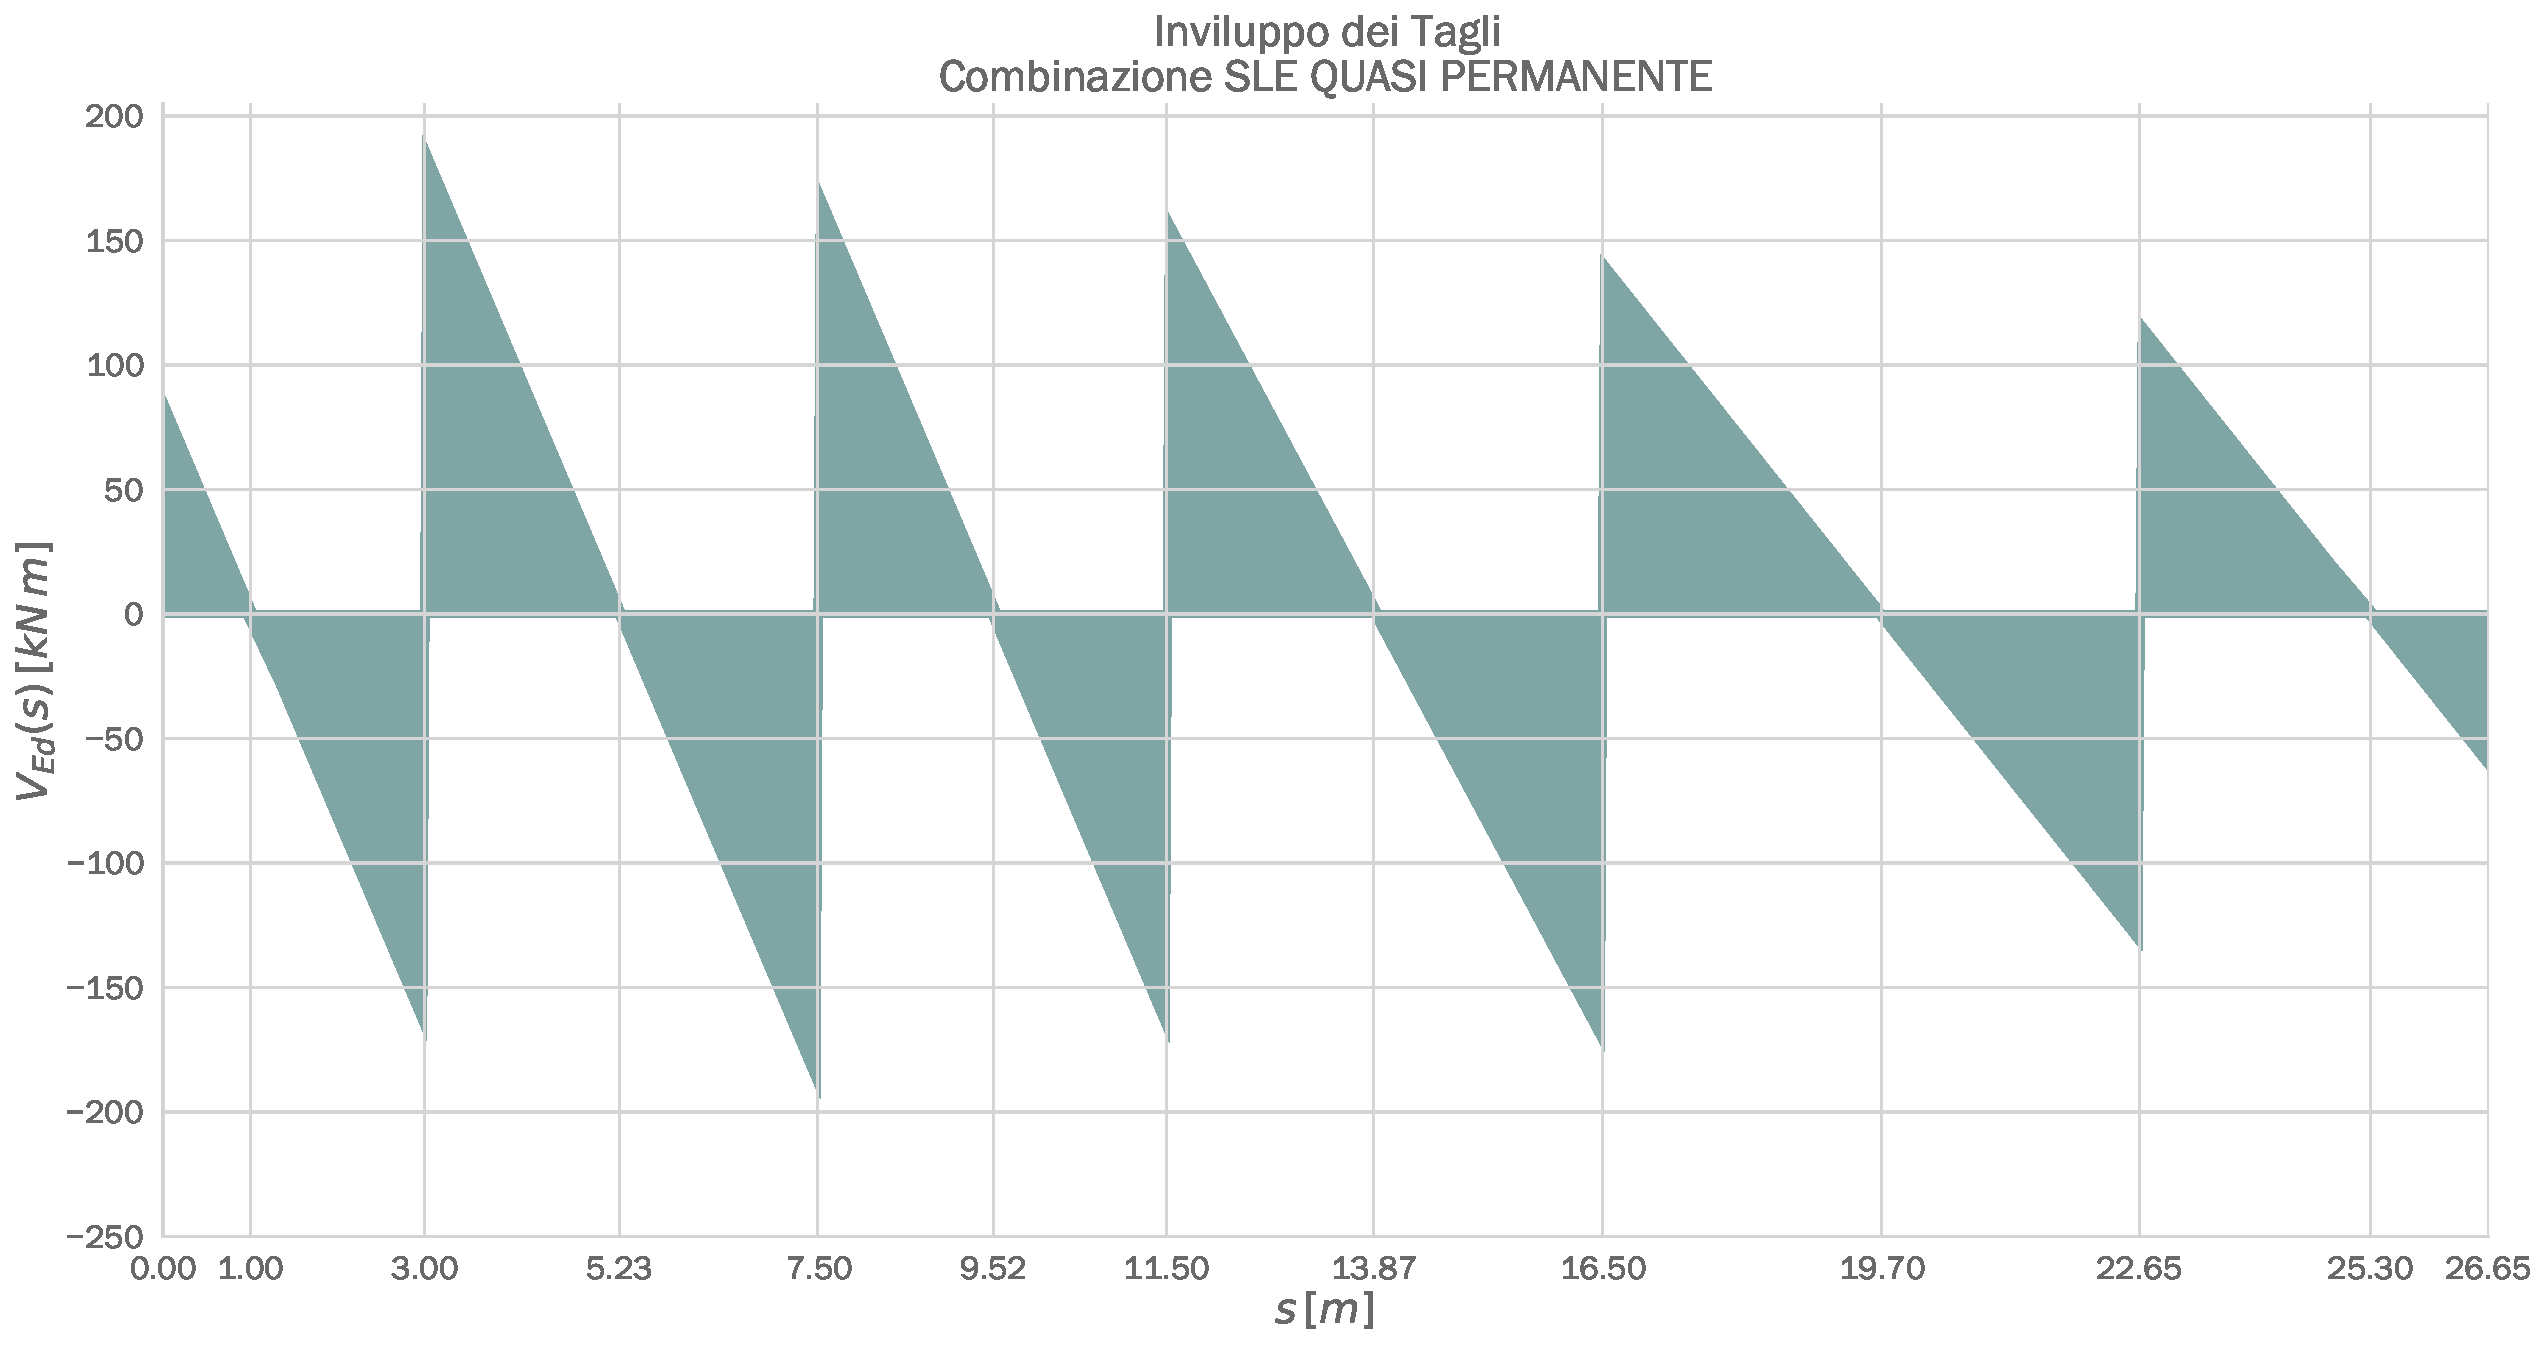
\includegraphics[width=.9\textwidth]{../../export/img/shearEnvelope_sleQP}}
	\caption{Diagrammi degli inviluppi per la combinazione SLE quasi permanente}
	\label{fig:envelope_sleQP}
\end{figure}

Termina qui l'analisi delle sollecitazioni agli stati limite per la trave. I valori delle tabelle, e le rispettive coordinate, verranno impiegati per l'armatura della trave, che non è direttamente trattata in questo documento.
\cleardoublepage
